% -*- program: xelatex -*-
\documentclass[11pt, compress]{beamer}
%\usepackage{listings}

\usepackage{pgfpages}

%\documentclass{article}
%\usepackage{beamerarticle}

%\documentclass[12pt, compress]{beamer} 
%\documentclass[notes=only]{beamer}

\usepackage{fontspec}

\setsansfont{PT Sans}
\setmonofont{PT Mono}

\usepackage{beamerthemesplit}
\usefonttheme[onlymath]{serif}
%\DeclareFontEncoding{T1}
\fontencoding{T1}

%\usepackage[T2A]{fontenc}
%\usepackage[utf8]{inputenc}
\usepackage[russian]{babel}
\usepackage{listings}


\usepackage{amsmath,amssymb,amsthm}
\hypersetup{unicode=true}

\usepackage{color}
\definecolor{mygred}{RGB}{150,0,0} 
\definecolor{mygreen}{RGB}{28,172,0} 
\definecolor{mylilas}{RGB}{170,55,241}
\definecolor{codecolor}{RGB}{0,120,0}
\definecolor{emphcolor}{RGB}{0,0,120}
\definecolor{gray}{RGB}{150,150,150}

\definecolor{light-gray}{gray}{0.95}
\definecolor{light-green}{rgb}{0.93, 1, 0.8}
\definecolor{light-yellow}{rgb}{1,1,0.85}
\definecolor{light-red}{rgb}{0.8, 0.3, 0.3}

\definecolor{dark-blue}{rgb}{0,0,0.6}
\definecolor{dark-red}{rgb}{0.7,0.0,0.0}
\definecolor{dark-green}{RGB}{10,150,0}

\usepackage{pifont}% http://ctan.org/pkg/pifont
\newcommand{\cmark}{\textcolor{green}{\ding{51}}}
\newcommand{\xmark}{\textcolor{red}{\ding{55}}}

\newcommand{\matcode}[1]{ \textcolor{codecolor}{\texttt{#1}}}
\usepackage{graphics,graphicx}
\usepackage{verbatim}
\usepackage{fancyvrb}
\usepackage{booktabs}
%\usepackage{media9}

\usepackage[super]{natbib}
 
\newcommand{\cleartitlepage}[1]{\begin{frame}[plain]\begin{center}\textsc{#1}\end{center}\end{frame}}

\renewcommand{\emph}[1]{\textcolor{emphcolor}{#1}}
\newcommand{\emphb}[1]{\textcolor{emphcolor}{\textbf{#1}}}


\usetheme{CambridgeUS}
\usecolortheme{lily}

\usepackage{tikz}
\usetikzlibrary{positioning} 
\tikzset{cbutton/.style={rectangle,minimum width=10mm,thick,draw=red!50!black!50,
top color=white,bottom color=red!50!black!30}}
\tikzset{mbutton/.style={rectangle,minimum width=10mm,thick,draw=black!20,
top color=white,bottom color=black!30}}


\lstset{basicstyle=\ttfamily\footnotesize,
    language=Python,    
    keepspaces=true,
    extendedchars=true,
    basicstyle={\footnotesize  \color{black}},
    breaklines=true,    
    keywordstyle=\color{blue},
    morekeywords=[2]{1}, keywordstyle=[2]{\color{codecolor}},
    identifierstyle={ \bf \color{black} },
    stringstyle=\color{mylilas},
    commentstyle=\color{mygreen},%
    showstringspaces=false,
    numbers=left,%
    numberstyle={\tiny \color{black}},
    numbersep=7pt, 
    emph=[1]{case,switch,otherwise},emphstyle=[1]\color{blue}, 
    frame=single,    
    rulecolor=\color{red},    
    backgroundcolor=\color{light-gray},
    xleftmargin=0.3cm,
    frame=l,framesep=4pt,framerule=0.5pt,
    showspaces=false,
    escapechar=|
    %lineskip=-0.3pt,
    %emph=[2]{word1,word2}, emphstyle=[2]{style},    
}

\setbeamertemplate{blocks}[rounded][shadow=false]
\setbeamertemplate{navigation symbols}{}

\makeatother
\setbeamertemplate{footline}
{
  \leavevmode%
  \hbox{%
  \begin{beamercolorbox}[wd=.3\paperwidth,ht=2.25ex,dp=1ex,center]{author in head/foot}%
    \usebeamerfont{author in head/foot}\insertshortauthor
  \end{beamercolorbox}%
  \begin{beamercolorbox}[wd=.6\paperwidth,ht=2.25ex,dp=1ex,center]{title in head/foot}%
    \usebeamerfont{title in head/foot}\insertshorttitle
  \end{beamercolorbox}%
  \begin{beamercolorbox}[wd=.1\paperwidth,ht=2.25ex,dp=1ex,center]{date in head/foot}%
    \insertframenumber{} / \inserttotalframenumber\hspace*{1ex}
    %\insertframenumber{} \hspace*{0.1ex}
  \end{beamercolorbox}}%
  \vskip0pt%
}


% define colours
% taken from pickton on Adobe Kuler:
% https://kuler.adobe.com/Some-Kind-Of-Execushares-color-theme-3837185/
 \definecolor{ExecusharesRed}{RGB}{230,37,52}
 \definecolor{ExecusharesBlack}{RGB}{43,40,40}
 \definecolor{ExecusharesBlue}{RGB}{22,190,207}
 \definecolor{ExecusharesWhite}{RGB}{255,255,243}
 \definecolor{ExecusharesGrey}{RGB}{107,110,108}

% \setbeamertemplate{itemize item}{
%  \tikz{
%    \draw[fill=emphcolor,draw=none] (0, 0) rectangle(0.1, 0.1);
%    \draw[fill=emphcolor,draw=none] (0.1, 0.1) rectangle(0.2, 0.2);
%    \draw[fill=emphcolor,draw=none] (0, 0.2) rectangle(0.1, 0.3);
%  }
% }

\AtBeginSection[]{
  \begin{frame}[plain]
  %\vfill  
  \begin{tikzpicture}
  \useasboundingbox (0,0) rectangle(\the\paperwidth,\the\paperheight);  
  \fill[color=mygred]   (-1cm, 3.9cm) rectangle(\the\paperwidth, 5.9cm);
  %\usebeamerfont{title}\insertsectionhead\par%
  %\node[text width=\the\paperwidth,align=center] at (current page.center) {\color{ExecusharesWhite}\Large\textbf{\insertsectionhead}};  
  \node[text width=\the\paperwidth,align=center] at (6cm,4.9cm) {\color{ExecusharesWhite}\Large\textbf{\insertsectionhead}};  
  \end{tikzpicture}
  \end{frame}
}

\setbeamertemplate{headline}{}
\setbeamertemplate{footline}{}

\makeatother
\setbeamertemplate{footline}
{
  \leavevmode%
  \hbox{%  
  \begin{beamercolorbox}[wd=.3\paperwidth,ht=2.25ex,dp=1ex,center]{author in head/foot}%
    \usebeamerfont{author in head/foot}\insertshortauthor
  \end{beamercolorbox}%  
  \begin{beamercolorbox}[wd=.6\paperwidth,ht=2.25ex,dp=1ex,center]{title in head/foot}%
    \usebeamerfont{title in head/foot}\insertshorttitle
  \end{beamercolorbox}%
  \begin{beamercolorbox}[wd=.1\paperwidth,ht=2.25ex,dp=1ex,center]{date in head/foot}%
    \insertframenumber{} \hspace*{1ex}
  \end{beamercolorbox}}%
  \vskip0pt%
}

\setbeamercolor{frametitle}{fg=dark-red,bg=gray!10}
\setbeamerfont{title}{series=\bfseries,parent=structure}
\setbeamerfont{frametitle}{series=\bfseries,parent=structure}

\usepackage{media9}

\definecolor{dark-blue}{rgb}{0,0,0.6}
\definecolor{dark-red}{RGB}{204,0,0}
\definecolor{dark-green}{RGB}{28,172,0}

\lstset{language=Matlab,    
    keepspaces=true,
    extendedchars=true,
    basicstyle={\footnotesize  \color{black}},
    breaklines=true,
    morekeywords={matlab2tikz},
    keywordstyle=\color{blue},
    morekeywords=[2]{1}, keywordstyle=[2]{\color{codecolor}},
    identifierstyle={ \bf \color{black} },
    stringstyle=\color{mylilas},
    commentstyle=\color{mygreen},%
    showstringspaces=false,
    numbers=left,%
    numberstyle={\tiny \color{black}},
    numbersep=7pt,  
    emph=[1]{case,switch,otherwise},emphstyle=[1]\color{blue}, 
    frame=single,    
    %lineskip=-1.0pt,
    %emph=[2]{word1,word2}, emphstyle=[2]{style},    
}

\title{Файл-функции и скрипты}
\subtitle{Основы MATLAB}
\author[Кафедра теоретической механики]{Юдинцев В. В.}
\small
\institute{Кафедра теоретической механики}

\begin{document}

{
\usebackgroundtemplate{
\includegraphics[width=\paperwidth,height=\paperheight]{back.png}}
\begin{frame}[plain]
\maketitle
\end{frame}
}
%\section[Содержание]{} 
\frame{
\frametitle{Содержание}
\tableofcontents
}



\section{Функции пользователя}

\begin{frame}[fragile]{Способы задания функции}
  \begin{itemize}
   \item inline функции;
   \item анонимные функции;
   \item файл-функции.
  \end{itemize}
\end{frame}

\begin{frame}[fragile]{inline-функция}  
\begin{lstlisting}
>> f1 = inline('x1^2+x2^2','x1','x2');
>> f1(4,2)
ans = 
   20
\end{lstlisting}
\alert{Переменные из рабочей области недоступны}.
\end{frame}

\begin{frame}[fragile]
  \frametitle{Анонимная функция}
\begin{lstlisting}
>> f = @ (x1,x2) x1^2+x2^2;  
>> f(4,2)
ans =
   20
\end{lstlisting}
Переменные из рабочей области доступны, но рассматриваются как константы:
\begin{lstlisting}
>> a=2;
>> f = @ (x1) a*x1;
>> f(1)
ans =
   2
>> a=1; f(1)
ans =
   2
\end{lstlisting}  
\end{frame}

%\begin{frame}[containsverbatim]{Экспорт данных}
%  Экспорт данны в файл csv  
%\end{frame}

%\begin{frame}[containsverbatim]{Импорт данных}
%  Экспорт данны в файл csv  
%\end{frame}

\section{Файлы-функции и скрипты}

\frame
{
  \frametitle{Типы файлов}  
  \begin{itemize}
    \item \matcode{*.m} (текстовые) содержат тексты программ, определения функций.
    \item \matcode{*.mat} (бинарные) содержат значения переменных.
    \item \matcode{*.mex} (бинарные). MEX-файлы -- динамически подключаемые библиотеки
  \end{itemize}
}

\begin{frame}[fragile]{Скрипты}      
    \begin{itemize}
      \item Любую последовательность команд в MATLAB можно оформить в виде m файла.
      \item По умолчанию все переменные, объявленные внутри файл-скрипта, являются глобальными.
    \end{itemize}
\end{frame}

\begin{frame}[fragile]{Функции}    
      \begin{itemize}
	\item Файл-функция содержит определение одной или нескольких функций. 
	\item По-умолчанию все переменные, объявленные внутри файл-функции, являются локальными. 
	\item Файл-функция является самостоятельным программным модулем, который связан с другими модулями и головной программой через входные и выходные параметры.
      \end{itemize}  
\end{frame}

\begin{frame}[fragile]{Создание m-файлов}
\begin{itemize}
\item При создании файл-функций и файл-скриптов следует избегать перекрытия имён других функций.
\item Для проверки имени можно использовать функцию \matcode{exist}:
\begin{lstlisting}
>> exist atan
ans =
     5 
\end{lstlisting}
\item Если имя не занято, то функция \matcode{exist} возвращает 0 (5 -- если имя занято встроенной функцией). 
\end{itemize}
\end{frame}
%
%
\section{Файл-скрипты}
%
%
\frame[containsverbatim]
{
  \frametitle{Файл-скрипт}  
  \begin{itemize}
  \item Файл-скрипт не имеет входных и выходных аргументов.
  \item Работает с данными из рабочей области.
  \item Все переменные, объявленные в файл-скрипте, являются глобальными.
  \item В процессе выполнения не компилируются.
  \item Представляют собой зафиксированную в виде файла последовательность операций.  
  \end{itemize}
}

\begin{frame}[fragile]{Структура файл-скрипта}  
Файл {\tt fscript.m}
\begin{lstlisting}
  % Описание кода,
  % которое можно увидеть
  % напечатав help fscript в окне команд
  x=1:0.1:10;
  y=sin(x);
\end{lstlisting}
\end{frame}


\begin{frame}[fragile]{Выполнение файл-скрипта}
  \begin{itemize}
   \item Вызов из командной строки (command window)
   \item Запуск из редактора при помощи сочетания  \tikz \node [cbutton] {Ctrl}; \tikz \node [cbutton] {Enter};
   \item Файл-скрипт можно для удобства разделить на ячейки (секции) при помощи удвоенного знака \matcode{\%\%}
  \begin{Verbatim}[formatcom=\color{codecolor}]
  %% секция 1
  код ...
  %% секция 2
  код ...
  \end{Verbatim}
  \item Код в каждой секции может быть выполнен при помощи \\ \tikz \node [cbutton] {Ctrl}; \tikz \node [cbutton] {Enter};
  \end{itemize}
\end{frame}
% 
%
\section{Файл-функции}
%
%
\begin{frame}[fragile]{Объявление функции}  
  \tikz \node [mbutton] {File}; \tikz \node [mbutton] {New}; \tikz \node [mbutton] {Function};
  \begin{lstlisting}
  % комментарии к функции, 
  % которые будут выводится 
  % по команде
  % help func_name
  function [out1,out2] = func_name(in1,in2)
   %
   % тело функции
   %
   out1=...
   out2=...
  \end{lstlisting}
\end{frame}

\begin{frame}[fragile]{Глобальные переменные в функциях}
  \begin{itemize}
    \item По умолчанию все переменные внутри функции являются локальными.
    \item Для того, чтобы несколько функций использовали одну переменную, её необходимо объявить глобальной.
  \end{itemize}
\begin{lstlisting}
  function res = func_name(in1,in2)
   global G; 
   res=G*in1+in2;   
\end{lstlisting}
\end{frame}


\begin{frame}[fragile]{Выполнение функций и файл-скриптов}
  Имя файла и имя объявленной в нем функции предпочтительно делать одинаковыми.
  Каталог, в котором содержатся вызываемые функции, должен быть текущим или добавлен в пути поиска.
  \begin{figure}[ht]
    \centering
    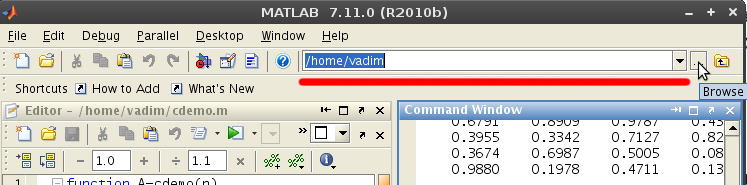
\includegraphics[width=10cm]{./dir.png}
  \end{figure}
\end{frame}

\frame[containsverbatim]
{
  \frametitle{Выполнение функций и файл-скриптов}
  \tikz \node [mbutton] {File}; \tikz \node [mbutton] {Set Path};
  \begin{figure}[ht]
    \centering
    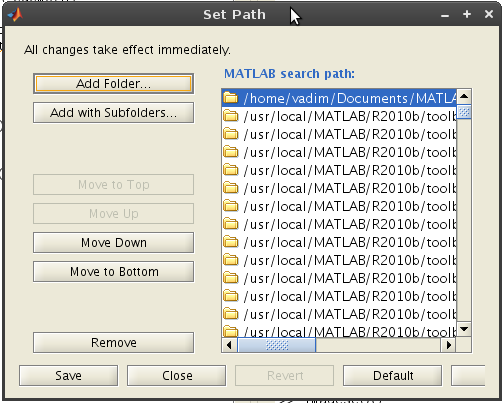
\includegraphics[width=5cm]{./setpath.png}
  \end{figure}
}

\frame[containsverbatim]
{
  \frametitle{Оператор return}  
  \begin{itemize}
   \item Функция прекращает работу после выполнения последнего оператора.
   \item Принудительно завершить функцию можно оператором \matcode{return}.
  \end{itemize}
}

\begin{frame}[fragile]{Быстрое построение графика функции}
\begin{columns}
\column{0.6\linewidth} 
\begin{center}
 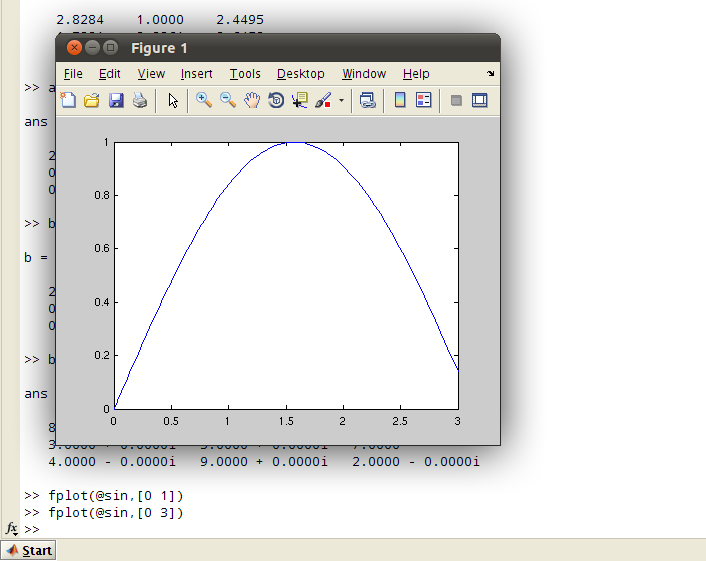
\includegraphics[width=1\linewidth]{./fplot.png}
\end{center}
\column{0.4\linewidth} 
Функция \matcode{fplot} \\
\begin{lstlisting}
fplot('myfun',[0 4])
fplot(@myfun,[0 4]) 
\end{lstlisting}
первый аргумент: имя или ссылка на функцию, второй аргумент: диапазон изменения аргумента функции для построения графика
\end{columns}
\end{frame}

\begin{frame}[fragile]{Внутренние функции}
\begin{itemize}
\item Файл-функция вместе с определением основной функции может содержать определения вспомогательных функций, доступных к вызову только из основной функции. 
\begin{lstlisting}     
function f = myfun(x)
  f1=infun(x);
  f=f1+cos(x);
% Внутренняя функция
function f = infun(x)
  a=3;
  f=sin(x*3);
\end{lstlisting}
  \item Переменные, используемые в подфункциях \emph{локальные}.
\end{itemize}  
\end{frame}

\begin{frame}[fragile]{Вложенные функции}
\begin{itemize}
\item Вложенная функции определяется в теле основной функции. \\
Файл {\tt myfun.m}:
\begin{lstlisting}
function f = myfun(x)
  f1=infun(x);
  f=f1+cos(x);
  function f = infun(x)
    f=sin(x);
  end
end    
\end{lstlisting}
 \item Из вложенной функции \matcode{infun} доступны локальные переменные всех функций верхнего уровня и наоборот.
\end{itemize}
\end{frame}

\begin{frame}[fragile]{Функции c переменным количеством аргументов}
\begin{itemize}
  \item \matcode{varargin} -- список ячеек с параметрами функции;
  \item \matcode{length(varargin)} -- количество переданных аргумента;
  \item \matcode{varargin\{1\}} -- первый аргумент;
  \item \matcode{varargin\{2\}} -- второй аргумент.
\end{itemize}  
\begin{lstlisting}
function res = fun(varargin)
  if length(varargin)<2
    error('Недостаточное количество аргументов');
  end
  ...
\end{lstlisting}
\end{frame}

\begin{frame}[fragile]{Функции c переменным количеством аргументов}
Аргумент \matcode{varargin} может быть указан после перечня обязательных аргументов 
\begin{lstlisting}
function res = fun(a1,a2,varargin)
  if length(varargin)<4
    error('Недостаточное количество аргументов');
  end
  ...
\end{lstlisting}
\end{frame}


\begin{frame}[fragile]{Функция в качестве аргумента}
Использование функции \matcode{feval}

Передача имени функции строкой:
\begin{lstlisting}
>> x = 1;
>> feval('sin',x)
ans =
    0.8415
\end{lstlisting}

Передача ссылки на функцию (это работает быстрее):
\begin{lstlisting}
>> feval(@sin,x)
ans =
    0.8415
\end{lstlisting}
\end{frame}

%
%
% \section{Задачи}
%
%
%
% \begin{frame}[fragile]{Конечные разности}
% Дана таблично-заданная функция $y(x)$ на равномерной сетке, например:\\
% \matcode{x=[0.1 0.2 0.3 0.4 0.5 0.6 0.7];}\\
% \matcode{y=[0.3 0.7 0.6 0.2 0.3 0.1 -0.5];}

% Построить матрицу конечных разностей вида
%   $$
%   \begin{pmatrix}
%    y_0 & \Delta y_0 & \Delta^2 y_0 & \ldots & \Delta^n y_0 \\
%    y_1 & \Delta y_1 & \Delta^2 y_1 & \ldots & 0 \\
%    \ldots & \ldots & \ldots & \ldots & 0 \\
%    y_n & \Delta y_n & 0 & \ldots & 0 
%   \end{pmatrix}
%   $$
%   где $\Delta y_0 = y_1 - y_0, \, \Delta^2 y_0 = \Delta y_1 - \Delta y_0, \ldots$
% \end{frame}
 
% \begin{frame}[fragile]{Интервалы возрастания и убывания функции}
% \only<1>{
% Дана таблично-заданная функция $y(x)$:\\  
% \matcode{x=(0.12 0.20 0.41 0.60 0.74 0.82  0.89);}  
% \matcode{y=(0.30 0.70 0.61 0.20 0.31 0.10 -0.50);}  
% }

% Найти интервалы на которых функция убывает и интервалы на которых функция возрастает
% $$
%   r_{inc} = 
%     \begin{bmatrix} 
%     a_1 & b_1 \\ a_2 & b_2 \\ \ldots & \ldots \\ a_n & b_n 
%     \end{bmatrix}, \quad
%   r_{dec} = 
%     \begin{bmatrix} 
%     c_1 & d_1 \\ c_2 & d_2 \\ \ldots & \ldots \\ c_m & d_m 
%     \end{bmatrix}
% $$  
% \only<2>{Функция должна принимать или два аргумента \matcode{x} и \matcode{y} или один аргумент -- матрицу \matcode{xy} в в первом столбце (или в строке) которой находятся значния \matcode{x}, во втором столбце (или в строке) -- значения функции \matcode{y}.
% }
% \end{frame}

\end{document}
